\documentclass[aspectratio=169]{beamer} % for making videos 169 is inferior
\usepackage{graphicx}

\usetheme{AnnArbor}
\usecolortheme{XKDR}
\logo{
\includegraphics[width=1cm]{XKDR_Logomark_RGB_Full_Colour.png}}

\hypersetup{colorlinks,
    citecolor=blue,
    linkcolor=blue,
    anchorcolor=yellow
    }

\mode<presentation>
{
  \usetheme{boxes}
}

\usepackage[english]{babel}
\usepackage[latin1]{inputenc}
\usepackage{times}
\usepackage[T1]{fontenc}

\newcommand{\fullpage}[1]{
  \begin{frame}
    \vfill
    {\Large #1}
    \vfill
  \end{frame}
}

\addtobeamertemplate{navigation symbols}{}{%
    \usebeamerfont{footline}%
    \usebeamercolor[fg]{footline}%
    \hspace{1em}%
    {\large \insertframenumber/\inserttotalframenumber}
}

\usepackage[style=apa, citestyle=authoryear, bibstyle=numeric, natbib=true, backend=biber]{biblatex}
\addbibresource{regbibliography.bib}

\title{The unreasonable effectiveness of Julia}
\titlegraphic{
\includegraphics[width=2.88cm]{XKDR_Primary_Logo_RGB_Full_Colour.png}}
\author{Ayush Patnaik}

\hypersetup{pdfauthor   = Ayush Patnaik,
            pdftitle    = The unreasonable effectiveness of Julia,
            pdfsubject  = Julia effectiveness, 
            pdfkeywords = {Julia}
}

\begin{document}

\begin{frame}
  \titlepage
\end{frame}

\begin{frame}{Julia}
  Julia was born out of addressing the limitations of MATLAB and other high-level languages. 
  \begin{enumerate}
    \item To produce performant code in the existing frameworks, one had to resort to writing the heavy lifting code in other languages or opt for other ``inelegant'' solutions. 
    \item The existing scientific computing languages had proprietary code, limiting accessibility to their source code and imposing restrictions on customization and collaborative development.
  \end{enumerate}
  To supplant the existing framework, Julia had be to significantly better in terms of elegance, performance, and fostering a collaborative ecosystem. This became the core culture of Julia. 
  
\end{frame}

\begin{frame}[fragile]
  \frametitle{Installation}
  Julia multiplexer gets installed with just a single command. No \verb|sudo| required.  
  \begin{verbatim}
    curl -fsSL https://install.julialang.org | sh
  \end{verbatim}

  Everything is in the \verb|.julia| folder. 
  \begin{verbatim}
    ayush@woodpecker:~/.julia$ ls
    artifacts  environments  logs      registries
    compiled   juliaup       packages  scratchspaces
  \end{verbatim}

\end{frame}

\begin{frame}[fragile]
  \frametitle{Syntax}
  
  \begin{columns}[t]
  \column{0.5\textwidth}
  Variable declaration
  \begin{verbatim}
  a = 10
  b = 20
\end{verbatim}

Arithmetic operations
\begin{verbatim}
  sum = a + b
  product = a * b
  quotient = a / b
\end{verbatim}
Conditional statement
\begin{verbatim}
  age = 25
  if age >= 18
    println("You're an adult.")
  else
    println("You're a minor.")
  end
  \end{verbatim}
  
  \column{0.5\textwidth}
  Define a function
  \begin{verbatim}
  function greet(name)
    println("Hello ", name)
  end
\end{verbatim}
Call the function
\begin{verbatim}
  greet("Julia")
\end{verbatim}
Array creation
\begin{verbatim}
  numbers = [1, 2, 3, 4, 5]
\end{verbatim}
Loop through elements  
\begin{verbatim}
  for num in numbers
    println(num)
  end
  \end{verbatim}
  \end{columns}
  
  \end{frame}
%%%%%%%%%
  \begin{frame}[fragile]
    \frametitle{Syntax}
    \framesubtitle{Continued}

    \begin{columns}[t]
    \column{0.5\textwidth}
    List comprehension
    \begin{verbatim}
  squares = [i^2 for i in 1:5]
  \end{verbatim}
  
  Dictionary creation
  \begin{verbatim}
  person = Dict(
  "name" => "Alice",
  "age" => 30,
  "city" => "New York")
  \end{verbatim}
  Access values by key
  \begin{verbatim}
  person["name"])
    \end{verbatim}
    
    \column{0.5\textwidth}
  Create a matrix
\begin{verbatim}
  A = [1 2 3; 4 5 6; 7 8 9]
\end{verbatim}
Basic indexing
\begin{verbatim}
  element = A[2, 3]
  second_row = A[2, :]
  third_column = A[:, 3]
  submatrix = A[1:2, 2:3] 
\end{verbatim}
    Broadcasting example
    \begin{verbatim}
  A = [1 2 3; 4 5 6; 7 8 9]
  B = [2 2 2; 2 2 2; 2 2 2]
  C = A .+ B
  \end{verbatim}
    \end{columns}
    
    \end{frame}


\begin{frame}[fragile]
    \frametitle{Multiple Dispatch}
    \framesubtitle{Methods are selected based on all argument types}
    
    \begin{columns}[t]
        \column{0.5\textwidth}
        Define methods for different types
        \begin{verbatim}
function process(x::Number,
                 y::Number)
    return x + y
end

function process(x::String,
                 y::String)
    return x * y
end

function process(x::Array,
                 y::Array)
    return x .+ y
end
        \end{verbatim}

        \column{0.5\textwidth}
        Julia automatically selects correct method
        \begin{verbatim}
process(1, 2)         # 3
process("a", "b")     # "ab"
process([1,2], [3,4]) # [4,6]
        \end{verbatim}

        \vspace{0.3cm}
        \begin{itemize}
            \item No explicit method overloading needed
            \item Dispatch based on all arguments
            \item Compiler optimizes for each type combination
        \end{itemize}

    \end{columns}
    

\end{frame}

\begin{frame}[fragile]
    \frametitle{Multiple Dispatch in action}
    \framesubtitle{Same plot() function, different types}
    
    \begin{columns}[t]
        \column{0.48\textwidth}
        Vector plotting
        \begin{verbatim}
  using Plots
  x = range(0, 10, length=100)
  y = sin.(x)
  plot(x, y) 
        \end{verbatim}
        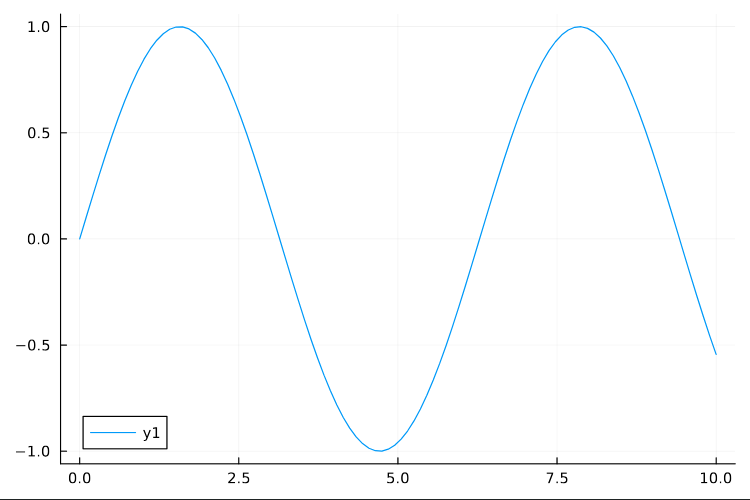
\includegraphics[width=0.8\textwidth]{sin_plot.png}
        
        \column{0.48\textwidth}
        Raster plotting
        \begin{verbatim}
  using Rasters
  A = Raster(WorldClim{BioClim},
             5)
  plot(A) 
        \end{verbatim}
        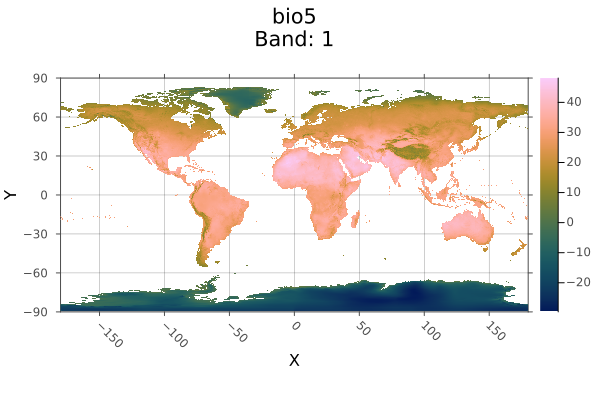
\includegraphics[width=0.9\textwidth]{raster_plot.png}
    \end{columns}
    
    \vspace{0.2cm}
    \begin{itemize}
        \item Same plot() function handles different types
        \item No explicit method selection needed
        \item Automatic dispatch to appropriate visualization
    \end{itemize}
\end{frame}

\begin{frame}[fragile]
  \frametitle{Package manager which doesn't fail}
  \vspace{0.5cm}  
  \begin{columns}[t]
  \column{0.5\textwidth}
  Adding a package
  \begin{verbatim}
  using Pkg
  Pkg.add("ExamplePackage")
  \end{verbatim}
  Updating packages
  \begin{verbatim}
  Pkg.update()
  \end{verbatim}
  \column{0.5\textwidth}
  Removing a package
  \begin{verbatim}
  Pkg.rm("ExamplePackage")
  \end{verbatim}
  Listing installed packages
  \begin{verbatim}
  Pkg.status()
  \end{verbatim}
  \end{columns}
\end{frame} 

\begin{frame}
  \hfill {\LARGE Thank you}.

  \vfill
  \vfill

  \hfill \url{https://xkdr.org}
\end{frame}

\begin{frame}[allowframebreaks]
  \frametitle{Bibliography}
  \renewcommand*{\bibfont}{\scriptsize}\printbibliography
\end{frame}

\end{document}
